\documentclass{article}

\usepackage[a4paper,margin=1in]{geometry}

\usepackage{mystyle}
\usepackage[sort,comma,numbers]{natbib}
\usepackage{algorithm}
\usepackage[noend]{algpseudocode}

\usepackage{subcaption}

\title{Storylines}

\begin{document}
\maketitle

\section{Introduction}
\begin{comment}
% Improve coherency of generative models of text by discovering a notion of storylines.
Our goal is to improve the coherency of generative story models by modeling storylines.
As an alternative to black-box models with little explicit structure,
prior work has noted that including structure in the generative model improves coherence
in the generations \citep{yao2018storyline,fan2019structure}.
However, prior investigations into narrative structure use hand-crafted representations,
such as entity coreference or keywords.
We hope to eventually alleviate the need for hand-crafted structure via structured generative models.

We first 
We perform an exploratory analysis of storyline induction by utilizing 
large pretrained sentence representations and alignment methods from biological sequence analysis.
We posit that 
\end{comment}

\section{Background: Pairwise Sequence Alignment}
The goal of pairwise sequence alignment is to find a minimum cost alignment
between sequences of sentences $\bx_1$ and $\bx_2\in\Sigma^*$, where
sentences are represented by a vector in $\R^n$.
We additionally add a gap symbol `-' to $\Sigma$, such that 
$\Sigma = \R^n \cup \set{-}$.
We refer to elements of $\Sigma$ as tokens.

In order to align two stories, pairwise alignment extends edit distance
with a distance measure $d: \Sigma\times\Sigma\to\R$ that operates on pairs of tokens,
one from each story.
The best alignment is given by the following:
\begin{equation}
\label{eqn:align}
\argmin_\pi \sum_{(i, j) \in \pi} d(x_{1,i},x_{2,j})
\end{equation}
where $\pi$ is a joint path through $\bx_1$ and $\bx_2$.
Valid paths are obtained by only inserting gaps into the original story
while preserving order.
Equation~\ref{eqn:align} can be solved exactly via dynamic programming.
Let $\bx^\pi_1,\bx^\pi_2$ be the gap-augmented stories obtained by following path $\pi$,
which are both of length $L$.
We refer to 
%\begin{equation}
$M = \begin{pmatrix}\bx^\pi_1 \\ \bx^\pi_2 \end{pmatrix}$
%\end{equation}
as the alignment.

When choosing a distance measure $d$, a key component is how the measure deals with gaps.
There are two approaches: 1) gaps correspond to insertion or deletions and 2) gaps
correspond to expansions or compressions.
Classical algorithms from biology, such as Needleman-Wunsch, model insertions and deletions,
as random mutations result in completely new elements that do not have a good interpretation
as an expansion or compression.
Time-series algorithms, such as Dynamic Time Warping (DTW), model expansions and compressions,
since warping may occur due to sampling at different frequencies or other reasons.
It is possible to model both of these in the distance measure.
For simplicity, we focus only on modeling insertion and deletion as this is a good
fit for story alignment:
Adding a sentence to a story, even if it builds on prior sentences,
adds new information.
% do I need to explain why?

\section{Problem Setup: Multiple Sequence Alignment}
In order to extract storylines, we would like to find patterns that are robust across
multiple stories. 
Unfortunately, methods for solving pairwise alignment are not directly applicable, since they
only consider pairs of stories.
Instead, we turn to the problem of multiple sequence alignment,
which generalizes alignment from pairs of stories to sets of stories.

Given a set of $K$ sequences,
a multiple alignment is a matrix $M \in \Sigma^{K \times L}$, given by:
\begin{equation}
M = \begin{pmatrix}
    \bx_1^\pi \\
    \vdots \\
    \bx_K^\pi
\end{pmatrix},
\end{equation}
where each $\bx_i^\pi$ is obtained by inserting gaps into the corresponding $\bx_i$
to ensure that each $\bx_i^\pi$ is of length $L$, as in pairwise alignment.

There are two common measures of quality for a multiple alignment:
1) the sum of pairs (SP) score and 2) the consensus error or Steiner distance.
In order to compute the SP score, we require a scoring function $d: \Sigma\times\Sigma\to\R$
that operates on pairs of tokens.
The SP score is given by
\begin{equation}
\mathrm{SP}(M) = \sum_{l=1}^L \sum_{i=1}^K \sum_{j=i+1}^K d(M_{il}, M_{jl}),
\end{equation}
obtained by summing the pairwise distances between elements of $M$ in the same column.

The consensus error given a consensus sequence $\bz\in\Sigma^L$ is defined as follows:
\begin{equation}
\mathrm{CE}(M, \bz) = \sum_{l=1}^L \sum_{i=1}^K d(M_{il}, z_{l}),
\end{equation}
the sum of the distances from each element in a column to $z_l$.
The mean sequence $\bz\in\Sigma^L$ that minimizes this error is known as the consensus sequence.

Finally, the Steiner distance is closely related to the consensus error,
and can be computed without explicitly constructing a multiple alignment.
Let $D: \Sigma^* \times \Sigma^* \to \R$
be the distance measure obtained under global pairwise alignment using the token distance $d$,
so that $D$ operates on pairs of sequences.
The Steiner distance is given by
\begin{equation}
\mathrm{SD}(\mcX, \bz) = \sum_{i=1}^K D(\bx_i, \bz).
\end{equation}
The optimal consensus error, $\min_\bz\mathrm{CE}(M,\bz)$,
is equivalent to the optimal Steiner distance, $\min_{\bz}\mathrm{SD}(\mcX, \bz)$
\citep{gusfield1997}.
Additionally, the optimal Steiner sequence, $\arg\min_{\bz}\mathrm{SD}(\mcX, \bz)$,
is equivalent to the optimal consensus sequence, $\arg\min_\bz\mathrm{CE}(M,\bz)$,
up to spaces.

We utilize algorithms that optimize both the SP score and the Steiner distance,
and report results on both.

\section{Methods}
As optimizing both the SP score and Steiner distance are NP-hard,
we resort to heuristic optimization methods.
We use a combination of three approaches: a progressive alignment method
inspired by a classical algorithm from computation biology,
an iterative averaging method similar to a popular algorithm from time-series analysis,
and a greedy hill climbing algorithm that operates in the space of Steiner sequences.

\subsection{Progressive Alignment}
Inspired by the progressive alignment algorithm
of \citet{fengdoolittle}, we first take a naive approach to approximating
a multiple sequence alignment.
Progressive alignments aim to optimize the SP score.

Given a set of sequences $\mcX$ and an ordering $\sigma$,
we progressively align the next sequence in the ordering to the
already aligned sequences.
Once a set of sequences are aligned, their columns of the alignment are frozen;
elements of new sequences must align to a whole column
from the existing alignment or a gap.
This is referred to as the `once a gap, always a gap' property \citep{fengdoolittle}.

In order to align a sequence to an existing alignment, we lift the definition of
the token distance $d$ to compare an element to a column of an alignment 
such that $d^+: \Sigma^*\times\Sigma\to\R$, as follows:
\begin{equation}
\label{eqn:dplus}
d^+(\by, x) = \sum_{j=1}^{|\by|} d(y_j, x).
\end{equation}
We can then extend pairwise global alignment with $d^+$, allowing us to
treat the columns of an alignment as if it were a token.
With the extended measure $d^+$, the full algorithm is given in Algorithm~\ref{alg:progressive}.

\begin{algorithm}[h]
\begin{algorithmic}
\State{Given: A set of sequences $\mcX = \set{\bx_i}_i$,
ordering $\sigma$, and extended distance measure $d^+$}
\State{Initialize alignment $M$ to $\bx_{\sigma(1)}$}
\ForAll{sequences $\bx_{\sigma(i)}$ in order $\sigma$}
    \State{Update $M = \Call{PairwiseAlign}{M, \bx_{\sigma(i)}, d^+}$ }
\EndFor
\Return{$M$}
\end{algorithmic}
\caption{\label{alg:progressive}
Progressive Alignment
}
\end{algorithm}

\subsection{An Iterative Averaging Algorithm}
Next, we propose an iterative averaging (IA)
algorithm which directly optimizes the Steiner distance.
The IA algorithm is inspired by the
DTW Barycenter Averaging (DBA) algorithm \citep{petitjean2011dba},
which iteratively computes pairwise alignments between a mean sequence $\bz$
and a set of sequences $\mcX$ then uses those alignments to recompute the mean sequence. 
As the DBA algorithm was designed to model expansion and compression, 
we adapt it for insertion and deletion.

The IA algorithm proceeds in a fashion similar to DBA.
We recompute the mean sequence by first constructing a multiple alignment from the
pairwise alignments, then for each column of the multiple alignment
computing the token that minimizes the distance to each element within that column.
As we model insertions and deletions,
there is ambiguity when mapping the pairwise alignments to a joint multiple alignment.
Namely, there are multiple ways of aligning tokens from $\mcX$ that are all to gaps.
We resolve this ambiguity heuristically by inserting gaps in
the $\bx_i^\pi$ obtained by pairwise alignment with $\bz$
so that all tokens aligned to elements in $\bz$ are aligned.
The algorithm is detailed in Algorithm~\ref{alg:ia}.

\begin{algorithm}[h]
\begin{algorithmic}
\State{Given: A set of sequences $\mcX = \set{\bx_i}_i$
and distance measure $d$}
\State{Given: Initial mean string $\bz$}

\Function{IterativeAverage}{$\bz, \mcX, d$}
\ForAll{iterations}
    \ForAll{sequences $\bx_i \in \mcX$}
        \State{Compute pairwise alignments $M^i = \Call{PairwiseAlign}{\bx_i, \bz, d}, M^i \in \Sigma^{2\times L_i}$}
    \EndFor
    \State{Compute multiple alignment $M = \Call{Stack}{M^1, \ldots, M^K}$}
    \State{Update $\bz = \Call{Average}{M, d}$}
\EndFor
\Return{$M$}
\EndFunction

\Function{Stack}{$M^1, \ldots, M^K$}
\While{Non-gap elements of $\bz$ are not aligned in all $M^i_2$}
\State{Record column indices of $M^i_2$ that have a non-gap element of $\bz$}
\State{Insert $(-,-)$ columns to the left of the columns with non-gap elements from $\bz$
    for each $M^i$}
\EndWhile
\Return{$\begin{pmatrix}M^{1}_1\\\hdots\\M^{K}_1\end{pmatrix}$}
\EndFunction

\Function{Average}{$M, d$}
\State{Initialize $\bz\in\Sigma^{L}$}
\ForAll{columns $l$ in $M$}
\State{Set proposal $z'$ to the average non-gap representation of column $l$}
\State{Compute cost $c(z') = \sum_i d(M_{il}, z')$ and $c(-) = \sum_i d(M_{il}, -)$}
\If{$c(z) > c(-)$}
\State{Set $z_l = -$}
\Else
\State{Set $z_l = z'$}
\EndIf
\EndFor
\Return{$\bz$}
\EndFunction

\end{algorithmic}
\caption{\label{alg:ia}
Iterative Averaging Alignment
}
\end{algorithm}

\subsection{Hill Climbing Algorithm}
As the previous iterative algorithm used a heuristic in the averaging step
that was computationally inexpensive but not guaranteed to improve the Steiner distance,
we also consider a greedy hill climbing (HC) algorithm that is more expensive but
guaranteed to improve the objective.

The hill climbing algorithm proceeds as follows: Given an initial mean sequence $\bz^{(0)}$,
we first compute the pairwise alignments from $\bz$ to each sequence in $\mcX$.
We obtain the first proposal sequence by averaging the token from each $\bx_i$ aligned
to each $z_t$.
Let this proposal be $\bz'$.
Next, we consider all proposals obtainable from one-step deviations
from $\bz'$, 
i.e. by adding or removing a single token.
To obtain the removal proposals, we simply consider removing each element of $\bz'$.
For the addition proposals, for each we take the average of the cartesian-product of tokens from each
$\bx_i$ aligned to a gap

\begin{algorithm}[h]
\begin{algorithmic}
\State{Given: A set of sequences $\mcX = \set{\bx_i}_i$,
and extended distance measure $d^+$}
\State{Initialize mean string $\bz$}
\ForAll{iterations}
    \ForAll{sequences $\bx_i \in \mcX$}
        \State{Compute pairwise alignments $M_i = \Call{PairwiseAlign}{\bx_i, \bz, d}$}
    \EndFor
    \State{compute proposal $\bz' = \Call{AverageAligned}{M_1,\ldots,M_{|\mcX|}}$}
    \State{}
    \ForAll{}
    \EndFor
    \ForAll{}
    \EndFor
    \State{Update $\bz = \Call{Average}{M}$}
\EndFor
\Return{$M$}
\end{algorithmic}
\caption{\label{alg:hillclimbing}
Hill Climbing Alignment
}
\end{algorithm}

\section{Experiments}
We evaluate our MSA approaches on the \textsc{WritingPrompts} dataset \citep{fan2018writingprompts},
a dataset of 300K human-written short stories obatined from the WritingPrompts subreddit.
Each story consists of a pair of a writing prompt and the story itself.
In our experiments, we use only the story.

We perform MSA on story sets of size 5.
As it would be intractable to run MSA on all story sets of size 5,
we use heuristics to select sets of stories that have low pairwise distance.
We use the following procedure to obtain the sets $\mcX$:
\begin{enumerate}
\item For every story in the \textsc{WritingPrompts} dataset,
we project each sentence using SBERT \citep{reimers2019sbert} into $\R^n$.
\item Compute bigram bag-of-sentence (BoS) representations of stories by
concatenating the SBERT representations of consecutive sentences, and averaging over time.
\item Take each of the first 50k stories from the \textsc{WritingPrompts} dataset as centroids,
and find 128 nearest neighbours for each in bigram BoS space.
\item Find the 4 closest stories to each centroid from its 128 neighbours
under the path-length normalized pairwise alignment distance.
We avoid selecting duplicates by discarding stories with matching 10-grams.
\item Select 50 centroids (and their closest stories), ensuring 
coverage over stories of different styles.
\end{enumerate}

For the token distance measure $d(x, y)$,
we use
\begin{equation} 
d(x,y) = \begin{cases}
0 & x=- \wedge y=-\\
\delta_x & x=- \wedge y\ne- \\
\delta_y & x\ne- \wedge y = -\\
\|x-y\|_2^2 & \mathrm{otherwise,}
\end{cases}
\end{equation}
where $\delta_x,\delta_y$ are the gap penalties.
This distance measure

When choosing the distance measure $d$, there are two key points:
1) whether to model insertions and deletions or compressions and expansions,
and 2) what token representation to operate on.
For 1) we focus on insertions and deletions, as they are a better fit for aligning
short stories about diverse topics. We are not concerned with identifying 
expansions upon the same story; we would like to find trends across somewhat
different stories.
For 2) we use 

In choosing clusters, as well as our experiments with progressive alignment,
we set $\delta_x=\delta_z \in \set{125, 150}$.
For the Steiner distance, we set $\delta_x \in \set{60, 75}$
and $\delta_y \in \set{180, 225, 300, 375}$.
We chose these gap penalties empirically based on preliminary analysis of the SBERT
nearest neighbours of sentences as well as the resulting multiple alignments.

We compare multiple alignments based on the SP score and Steiner distance,
and examine the output of each MSA algorithm by qualitatively evaluating the 
semantic closeness of alignments.
For computing the MSA, we use the progressive alignment, iterative averaging,
and hill climbing algorithm.
For the IA algorithm, we initialize the mean sequence with the longest sequence $\bx_i \in \mcX$.
For the hill climbing algorithm, we initialize the mean sequence with
either the mean sequence obtained from the progressive alignment or the IA algorithm,
yielding two configurations.

\section{Results}
We find that the MSA algorithms perform better on the objective they optimize,
as seen in Table~\ref{tbl:sp_steiner}.
The progressive alignment outperforms the other approaches by getting a lower SP score,
while the IA and hill climbing (initialized with the IA mean sequence)
approaches perform well on the Steiner distance.
Initializing the hill climbing approach with the mean sequence obtained from 
the progressive alignment results in an alignment that has a lower Steiner distance
than progressive, but the SP score increases.

\begin{table}
\centering
\begin{tabular}[h]{|l|c|c|c|c|}
\hline
\bf{Algorithm}              & $\delta_x$ & $\delta_y$ & \bf{SP Score} & \bf{Steiner Distance}\\
\hline
Progressive                 & 125        & 125        & 2,494,153.00  & 877,445.99 \\
Hill Climbing (Progressive) & 60         & 300        & 2,514,774.25  & 774,525.85\\
Iterative Averaging         & 60         & 300        & 2,643,249.25  & 716,350.33\\
Hill Climbing (IA)          & 60         & 300        & 2,647,854.25  & 709,076.44\\
\hline
\end{tabular}
\caption{
\label{tbl:sp_steiner}
The SP scores and Steiner distances for each of the MSA algorithms.
The progressive algorithm optimizes the SP score and achieves the lowest.
The hill climbing algorithm initialized with the mean sequence obtained from IA
obtains the lowest Steiner distance.
We see the algorithms get stuck in local optima, as the hill climbing algorithm
initialize with the progressive mean sequence obtains a much higher
Steiner distance than if it had been initialized with IA.
}
\end{table}

The alignments obtained from the Progressive alignments are longer and contain more gaps
than the hill climbing (IA) alignments.
This is shown in Figure~\ref{fig:colcounts},
where the total number of columns is much larger for progressive than HC(IA),
and the column densities are lower for progressive as well.
We hypothesize that this is due to the algorithms chosen for optimizing the Steiner distance.
In the IA algorithm, the gap penalty controls how the 
mean sequence accounts for the number of gaps within a column.
JK, need to think more about this still \citep{lei2004triangle}.

\begin{figure}
\begin{subfigure}{0.5\textwidth}
\centering
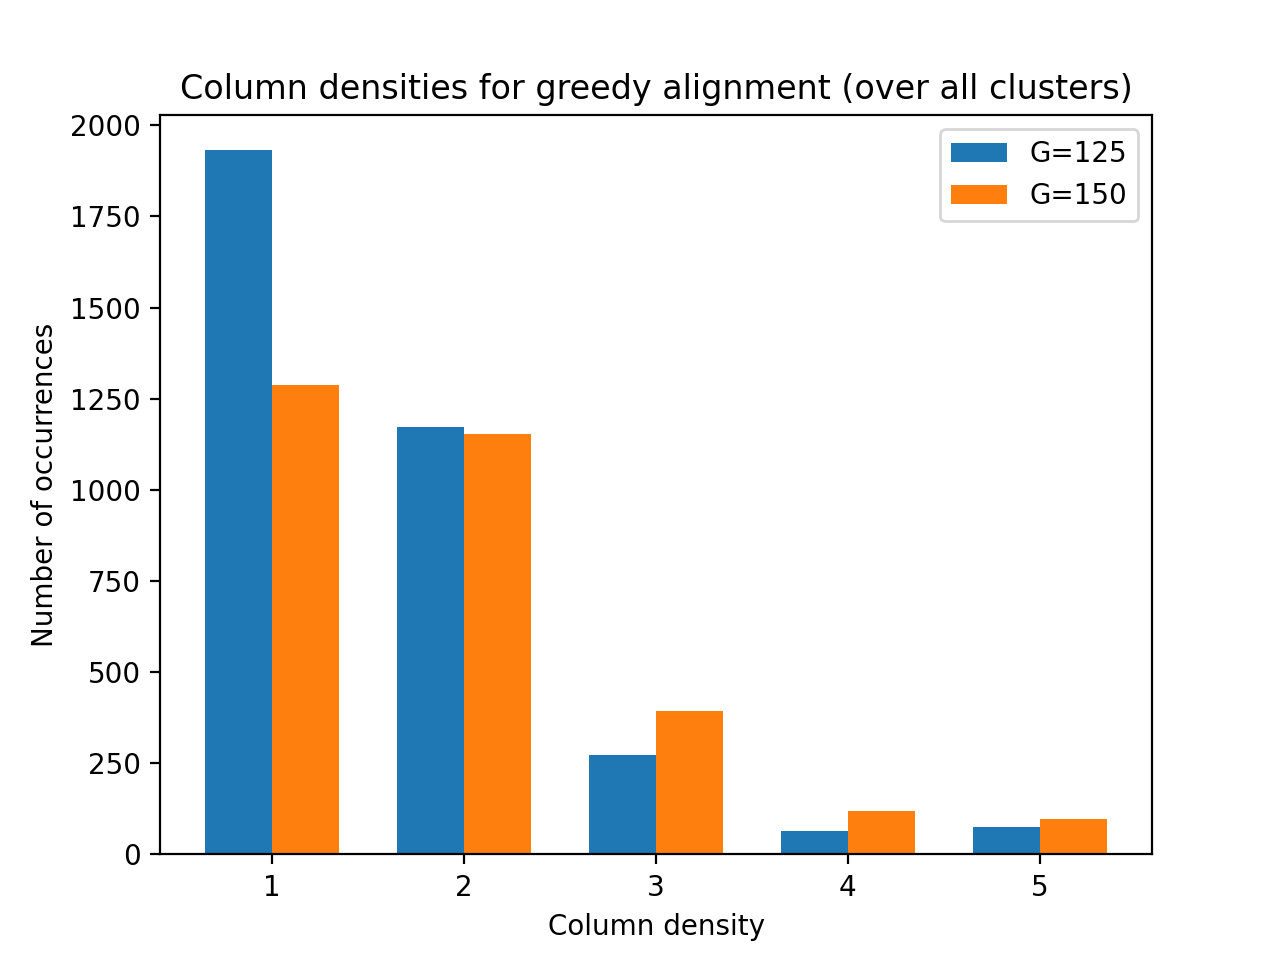
\includegraphics[width=3in]{img/prog125v150.png}
\caption{}
\end{subfigure}
\begin{subfigure}{0.5\textwidth}
\centering
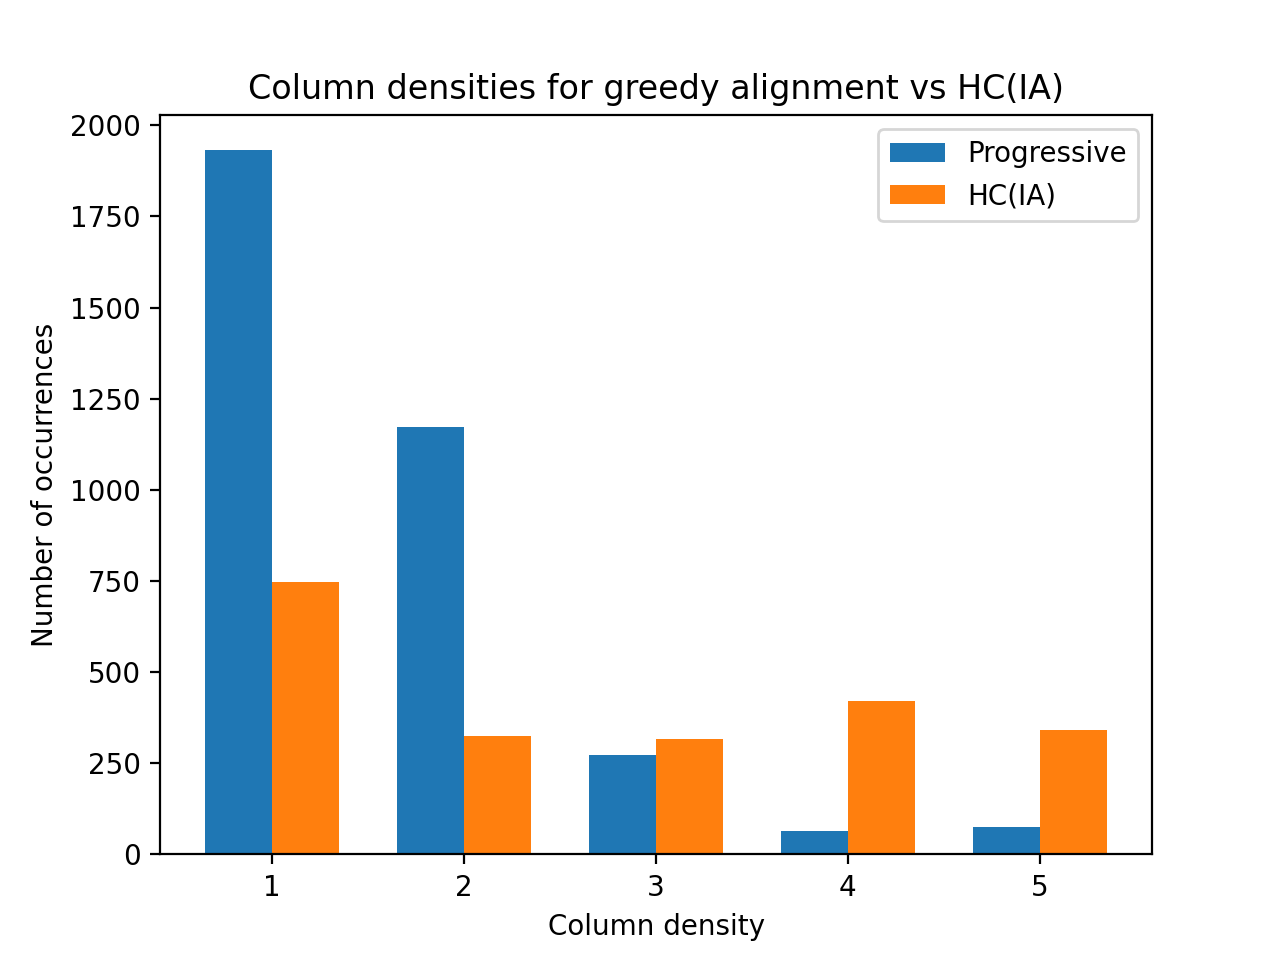
\includegraphics[width=3in]{img/prog125vhcia}
\subcaption{}
\end{subfigure}
\caption{
\label{fig:colcounts}
Merge into one graph.
}
\end{figure}




\newpage
\bibliographystyle{plainnat}
\bibliography{bib}

\end{document}
